\documentclass[pdftex,twocolumn,10pt,letterpaper]{article}
\setlength{\textheight}{9.0in}
\setlength{\columnsep}{0.25in}
\setlength{\textwidth}{6.50in}
\setlength{\topmargin}{0.0in}
\setlength{\headheight}{0.0in}
\setlength{\headsep}{0.0in}

\usepackage{hyperref}
\usepackage{graphicx}

\title{
    {
     Analysis of Co-locating Batch and Latency-critical\\
     Workloads in Single Cluster\\
     \large  CS 744 Spring 24 Project Proposal
    }
}
\author{Mondo Jiang, Zihao Zhu}
\date{}

\begin{document}

\maketitle

\section*{Introduction}
In this project, we plan to analyze different schedulers' behavior when scheduling low priority workloads (e.g. machine learning training jobs, daily conclution data analysis jobs, etc.)  and latency-critic workloads (e.g. web servers, machine learning inference and real-time interactive data analysis jobs) together in single cluster.

In previous works, most schedulers only schedule single type of workloads:
In Mesos, each workload has its own scheduler \cite{hindman2011mesos}, and INFaaS \cite{romero2021infaas} only considers machine learning inference workloads, etc. But we might achieve better resource utilization by having a centralized scheduler to manage various types of workloads. This is especially true in the case of webservices, because they always have idle resources during the day, as we can see in \autoref{fig:typical-day}.

\begin{figure}[h]
	\centering
	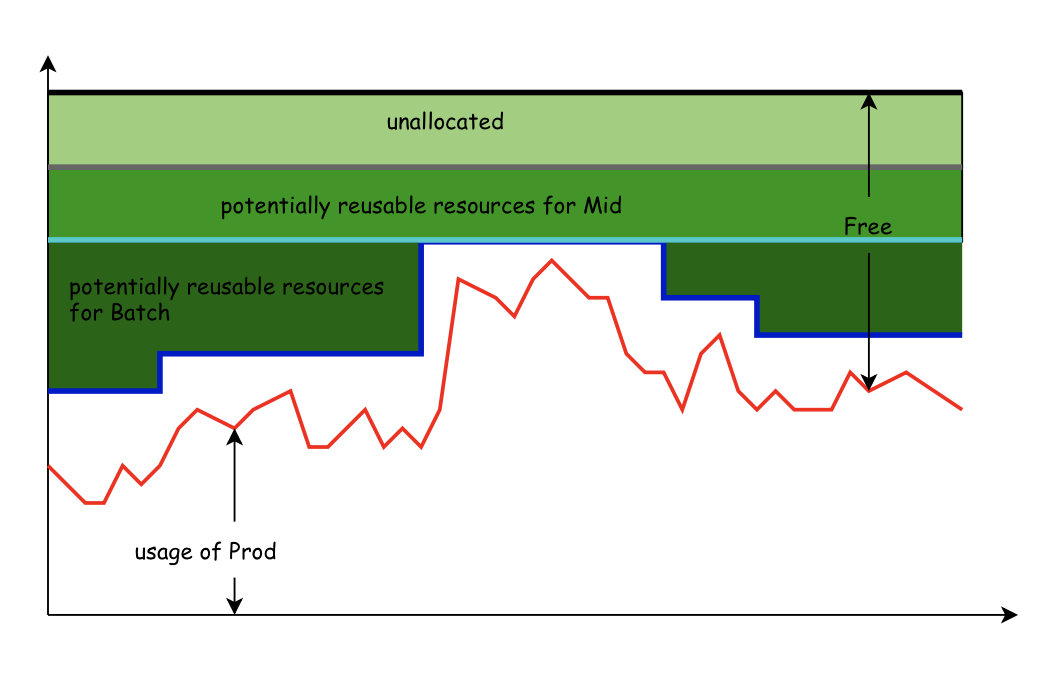
\includegraphics[width=0.5\textwidth]{fig/koo-time.png}
	\caption{A Typical Day of a Web Service \cite{koo}}
	\label{fig:typical-day}
\end{figure}

By co-locating batch jobs and real-time data analysis, we may further increase data locality among different jobs which manipute the same partition of data, and reduce the cost of data transfer. This is especially useful in cloud data center senerio, because it can significantly reduce the overall cost for running a data center.

We plan to use Koordinator \cite{koo} as our scheduler, and compare its performance with default K8s scheduler and other schedulers like Kube-Batch \cite{kube-batch}. We will also analyze the tide effect of different jobs (GPU and other resources), and how to give wiggle room for online jobs. Specifically, we will consider following use cases:

\begin{enumerate}
	\item co-locate webservices and batch jobs together in single cluster.
	      \begin{figure}[h]
		      \centering
		      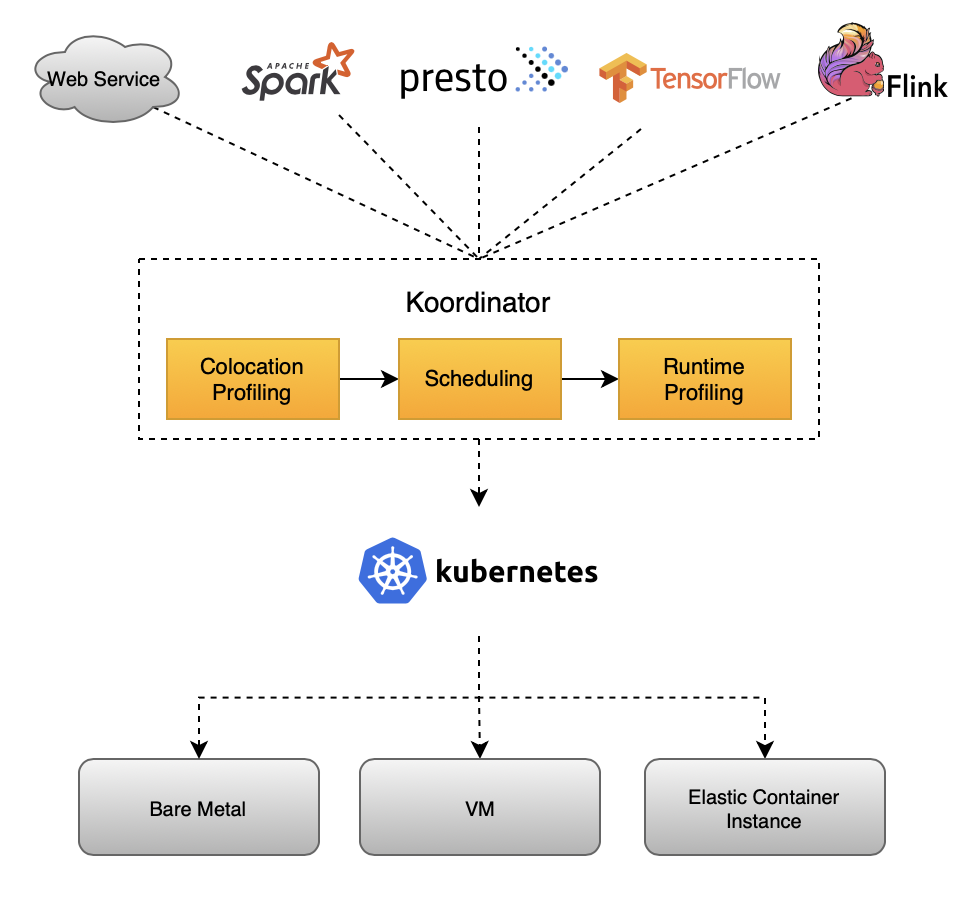
\includegraphics[width=0.5\textwidth]{fig/koo-arch.png}
		      \caption{Mixing Workloads in Single Cluster \cite{koo}}
	      \end{figure}
	\item running response time sensitive online ml models (gpt, search by image, receipt analysis) with batch processing and webservices.
	\item running real-time analytics on the same data that is used for batch processing to analyze locality traits.
\end{enumerate}

\section*{Methodology}

\begin{enumerate}
	\item Build a method to simulate different types of workloads in K8s (Web Services and its tide effect, Machine Learning Training and Inference Workloads, Hadoop Data Analysis Batch Jobs, Real-time Data Analysis).
	\item Compare between differently jobs performance in K8s using current schedulers, form the metrics (e.g. SLO for ML Inference and web server requests, total execution time for training and batch jobs, overall resource usage, etc.) and a baseline.
	\item Analysis more aspects of this topis, such as
	      \begin{enumerate}
		      \item Decisions made by current schedulers and their effects on cluster performance.
		      \item The tide effect of different jobs (GPU and other resources), how can we archive a overall better resource usage while not breaking SLO requirements.
		      \item How to give wiggle room for online jobs to handle fluctuation loads.
	      \end{enumerate}
	\item If time permits, we will also try to implement a new scheduler based on Kubernetes's default scheduler, and compare its performance with other schedulers.
\end{enumerate}

\section*{Timeline}


\section*{Related work}
\begin{description}
	\item [\href{https://kubernetes.io/docs/concepts/scheduling-eviction/kube-scheduler/}{Kube-Scheduler}] default scheduler for Kubernetes, supports scheduling based on resource requirements, Pod and Job correspond to different types of workloads.
	\item [\href{https://koordinator.sh}{Koordinator}] QoS-based scheduling for efficient orchestration of microservices, AI, and big data workloads on Kubernetes\cite{koo}
	\item [\href{https://github.com/kubernetes-retired/kube-batch}{Kube-Batch}] a batch scheduler for Kubernetes, providing mechanisms for applications which would like to run batch jobs leveraging Kubernetes.
	\item [\href{https://www.intel.com.br/content/dam/www/public/us/en/documents/white-papers/Intel_ByteDance_WhitePaper.pdf}{Bytedance Co-locate Practice with Intel}] Performance Evaluation and Optimization for Workload Colocation\cite{:aa}
\end{description}

{
\bibliographystyle{abbrv}
\bibliography{ref}
}

\end{document}
